\section{\trStraightening{}--\trUnstraightening}
\label{sec:straightening-unstraightening}

本节中，我们想要陈述并讨论一个重要的对应：\trGrothendieckConstruction{}。我们将要%
陈述并在一定程度上予以解释的主定理是\trLurie{}的\trStraightening{}--%
\trUnstraightening{}\trEquivalence{}，它把由一个固定∞-\trCategory{} $\mathcal{C}$
到∞-\trCategories{}的∞-\trCategory{}的\trFunctor{}所成的∞-\trCategory{}%
$\mathrm{Fun}(\mathcal{C}, \mathrm{Cat}_\infty)$，与 $\mathcal{C}$ 之上的%
\trCocartesianFibration{}的∞-\trCategory{}相比较。我们将详细解释如何把一个%
\trFunctor{} $\mathcal{C} \to \mathrm{Cat}_\infty$ 与 $\mathcal{C}$ 之上的一个%
\trCocartesianFibration{}联系起来，并且我们将简略陈述这一构造如何如上所述地构成%
∞-\trCategories{}之间\trEquivalence{}的一部分。此外，我们还将对这一\trEquivalence{}%
被设想如何产生给出一些概念性图景，并对何处可以找到对这一过程的分析给出一些文献指引。
我们指出，从一个\trCocartesianFibration{}出发构造\trFunctor{}%
$\mathcal{C} \to \mathrm{Cat}_\infty$ 的策略取自 \cite{Hau17}，其中对%
\trRightFibration{}的情形完成了这一变体。

我们从一个非正式的构造开始。考虑一个\trCocartesianFibration{}%
$p\colon \E \to \mathcal{C}$。由此，我们可以提取出下列数据：
\begin{enumerate}[label=(\arabic*)]
  \item 对 $\mathcal{C}$ 的每个\trObject{} $x$，我们有∞-\trCategory{} $\E_x$；
  \item 对 $\mathcal{C}$ 中的每个\trMorphism{} $f\colon x \to y$ 与 $\E_x$ 中的一个%
        \trObject{} $z$，我们可以选取 $f$ 的一个 $p$-余笛卡尔提升 $z \to w$，我们把它%
        记作 $w = f_!(z)$；
  \item 再给定 $\E_x$ 中一个\trObject{} $z'$ 与一个\trMorphism{}%
        $\alpha\colon z \to z'$，我们可以选取另一个 $p$-余笛卡尔提升
        $z' \to w' = f_!(z')$，从而得到图表
\begin{center}
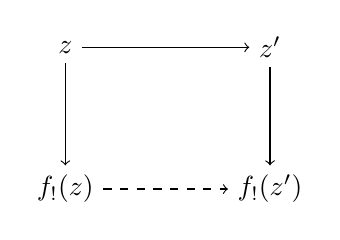
\begin{tikzpicture}
  \node (z) at (0,0) {$z$};
  \node (zp) at (2.6,0) {$z'$};
  \node (fz) at (0,-1.8) {$f_!(z)$};
  \node (fzp) at (2.6,-1.8) {$f_!(z')$};
  \draw[->] (z) -- (zp);
  \draw[->] (z) -- (fz);
  \draw[->] (zp) -- (fzp);
  \draw[->, dashed] (fz) -- (fzp);
\end{tikzpicture}
\end{center}
        由于 $z \to f_!(z)$ 是 $p$-余笛卡尔的，使图表交换的虚线箭头的空间是%
        \trContractible。我们把任何这样的虚线箭头记作 $f_!(\alpha)$。
\end{enumerate}

总结起来，与一个\trCocartesianFibration{} $p\colon \E \to \mathcal{C}$ 相联系的，
我们希望找到一个\trFunctor{} $\mathcal{C} \to \mathrm{Cat}_\infty$，它把一个%
\trObject{} $x$ 送到\trFibre{} $\E_x = p^{-1}(x)$，并把一个从 $x$ 到 $y$ 的%
\trMorphism{} $f$ 送到如上所示的一个\trFunctor{} $f_!\colon \E_x \to \E_y$。

\begin{proposition}\label{prop:pushforward-functor}
给定一个\trCocartesianFibration{} $p\colon \E \to \mathcal{C}$ 与一个从 $x$ 到 $y$
的\trMorphism{} $f\colon \Delta^1 \to \mathcal{C}$，存在一个\trFunctor{}%
$\E_x \times \Delta^1 \to \E$，它限制到 $\E_x$ 的每个\trObject{} $z$ 上给出 $f$
之上的一个 $p$-余笛卡尔\trMorphism{} $\alpha\colon z \to z'$。把这个\trFunctor{}%
限制到 $\E_x \times \{1\}$ 上便产生一个\trFunctor{} $f_!\colon \E_x \to \E_y$。
\end{proposition}

\begin{proof}
我们着手为每个\trCocartesianFibration{} $p\colon \E \to \mathcal{C}$ 与每个从 $x$
到 $y$ 的\trMorphism{} $f\colon \Delta^1 \to \mathcal{C}$ 构造一个\trFunctor{}%
$f_!\colon \E_x \to \E_y$。为此，回忆在这种情形下，由取\trMorphism{}的源给出的典范%
映射 $\mathrm{Fun}^{\mathrm{cc}}_f(\Delta^1, \E) \to \E_x$ 是一个%
\trTrivialFibration{}。选取这个\trTrivialFibration{}的一个\trSectionMap{}便产生复合
\[
f_!\colon \E_x \to \mathrm{Fun}^{\mathrm{cc}}_f(\Delta^1, \E) \to \E_y,
\]
其中后一个映射由取\trMorphism{}的目标给出。此外，我们发现第一个映射伴随于一个映射
\[
\E_x \times \Delta^1 \to \E,
\]
它具有下列性质：它限制到 $\E_x \times \{1\}$ 上由 $f_!$ 给出；它使图表
\begin{center}
\begin{tikzpicture}
  \node (exd) at (0,0) {$\E_x \times \Delta^1$};
  \node (e) at (3,0) {$\E$};
  \node (d1) at (0,-1.8) {$\Delta^1$};
  \node (c) at (3,-1.8) {$\mathcal{C}$};
  \draw[->] (exd) -- (e);
  \draw[->] (exd) -- (d1);
  \draw[->] (e) -- node[right] {$p$} (c);
  \draw[->] (d1) -- node[above] {$f$} (c);
\end{tikzpicture}
\end{center}
交换；而且，对 $\E_x$ 的每个\trObject{} $z$，所得的\trMorphism{} $\Delta^1 \to \E$
是一个源等于 $z$、目标等于 $f_!(z)$ 的 $p$-余笛卡尔\trMorphism{}。
\end{proof}

接下来，我们想证明对应 $f \mapsto f_!$ 在 $f$ 中是函子的。为此，我们考虑
$\mathcal{C}$ 内部的一个 $2$-\trSimplex{} $\sigma\colon \Delta^2 \to \mathcal{C}$，
它把 $h$ 展示为 $f$ 与 $g$ 的一个合成。那么，在图表
\begin{center}
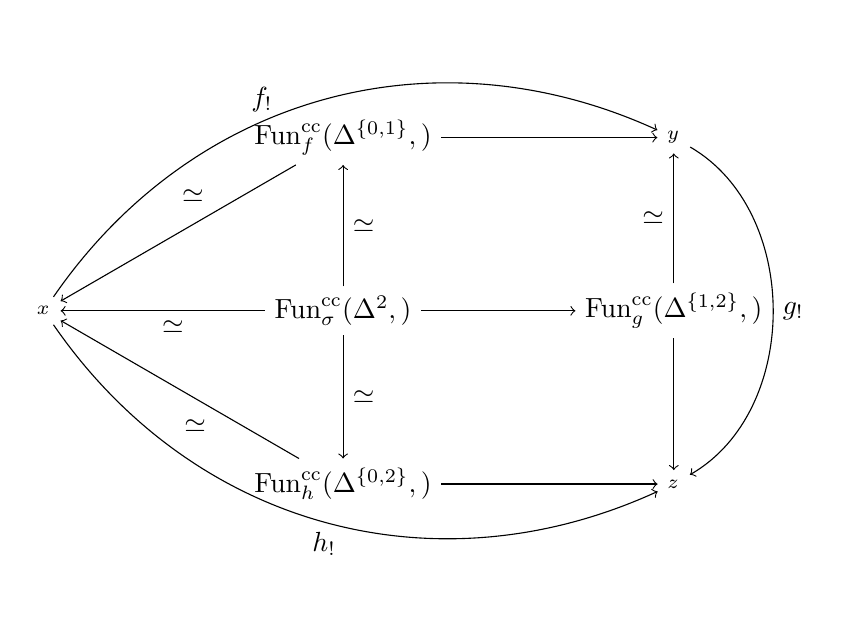
\begin{tikzpicture}
  \node (ex) at (0,-2.2) {$\E_x$};
  \node (funf) at (3.8,0)
    {$\mathrm{Fun}^{\mathrm{cc}}_f(\Delta^{\{0,1\}}, \E)$};
  \node (ey) at (8,0) {$\E_y$};
  \node (funs) at (3.8,-2.2) {$\mathrm{Fun}^{\mathrm{cc}}_\sigma(\Delta^2, \E)$};
  \node (fung) at (8,-2.2)
    {$\mathrm{Fun}^{\mathrm{cc}}_g(\Delta^{\{1,2\}}, \E)$};
  \node (funh) at (3.8,-4.4)
    {$\mathrm{Fun}^{\mathrm{cc}}_h(\Delta^{\{0,2\}}, \E)$};
  \node (ez) at (8,-4.4) {$\E_z$};
  \draw[->] (funf) -- (ey);
  \draw[->] (funf) -- node[above left, pos=0.35] {$\simeq$} (ex);
  \draw[->] (funs) -- node[right] {$\simeq$} (funf);
  \draw[->] (funs) -- node[below, pos=0.45] {$\simeq$} (ex);
  \draw[->] (funs) -- (fung);
  \draw[->] (fung) -- node[left] {$\simeq$} (ey);
  \draw[->] (funs) -- node[right] {$\simeq$} (funh);
  \draw[->] (funh) -- node[below left, pos=0.35] {$\simeq$} (ex);
  \draw[->] (funh) -- (ez);
  \draw[->] (fung) -- (ez);
  \draw[->] (ex) to[bend left=40] node[above, pos=0.4] {$f_!$} (ey);
  \draw[->] (ey) to[bend left=60] node[right, pos=0.5] {$g_!$} (ez);
  \draw[->] (ex) to[bend right=40] node[below, pos=0.5] {$h_!$} (ez);
\end{tikzpicture}
\end{center}
中，标有 $\simeq$ 的映射都是\trTrivialFibration{}，因为它们是沿%
\trLeftAnodyne{}映射的限制而出现的。这表明 $g_!f_!$ 与 $h_!$ 之间存在一个%
自然同构。

接下来，我们将解释一般的构造。为此，我们固定一个\trCocartesianFibration{}%
$p\colon \E \to \mathcal{C}$。

\begin{lemma}\label{lem:theta-functor}
把∞-\trCategory{} $\mathrm{Fun}^{\mathrm{cc}}_\sigma(\Delta^n, \E)$ 联系到
$\sigma\colon \Delta^n \to \mathcal{C}$ 的这一做法可扩充为一个\trFunctor{}%
$\Theta(p)\colon \Delta^{\mathrm{op}}_{/\mathcal{C}} \to \mathrm{sSet}$。
\end{lemma}

\begin{proof}
我们需要证明，一个交换图表
\begin{center}
\begin{tikzpicture}
  \node (dn) at (0,0) {$\Delta^n$};
  \node (dm) at (3.4,0) {$\Delta^m$};
  \node (c) at (1.7,-1.8) {$\mathcal{C}$};
  \draw[->] (dn) -- node[above] {$f$} (dm);
  \draw[->] (dn) -- node[below left] {$\sigma$} (c);
  \draw[->] (dm) -- node[below right] {$\tau$} (c);
\end{tikzpicture}
\end{center}
都诱导出一个良定义且具函子性的映射 $\mathrm{Fun}^{\mathrm{cc}}_\tau(\Delta^m, \E) \to \mathrm{Fun}^{\mathrm{cc}}_\sigma(\Delta^n, \E)$。而这一点由定义直接看出。
\end{proof}

\begin{definition}\label{def:W-X}
设 $X$ 是一个\trSimplicialSet{}。我们用 $W_X$ 表示 $\Delta_{/X}$ 中所有满足
$f(0) = 0$ 的\trMorphism{} $f\colon [n] \to [m]$ 所成之集。
\end{definition}

\begin{lemma}\label{lem:W-morphisms-joyal-equivalences}
设 $p\colon \E \to \mathcal{C}$ 是一个\trCocartesianFibration{}。那么\trFunctor{}%
$\Theta(p)$ 把 $W_\mathcal{C}$ 中的任何\trMorphism{}送到一个\trJoyalEquivalence{}。
\end{lemma}

\begin{proof}
考虑 $\Delta_{/\mathcal{C}}$ 中的一个\trMorphism{} $f$，它由复合
$\Delta^n \xrightarrow{f} \Delta^m \xrightarrow{\sigma} \mathcal{C}$ 所表示。
我们将记 $\tau = \sigma f$。由假设，复合
\[
\Delta^{\{0\}} \to \Delta^n \xrightarrow{f} \Delta^m
\]
挑出 $\Delta^m$ 中的\trObject{} $0$。于是，我们有交换图表
\begin{center}
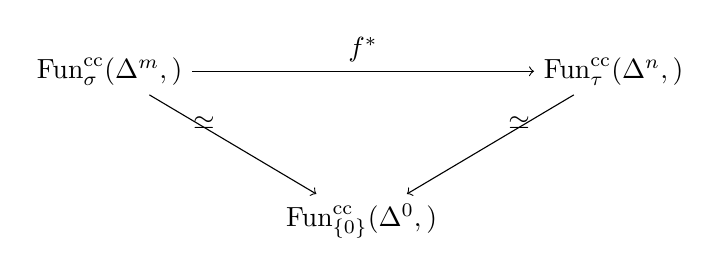
\begin{tikzpicture}
  \node (ms) at (0,0) {$\mathrm{Fun}^{\mathrm{cc}}_\sigma(\Delta^m, \E)$};
  \node (ns) at (6.4,0) {$\mathrm{Fun}^{\mathrm{cc}}_\tau(\Delta^n, \E)$};
  \node (zero) at (3.2,-1.9) {$\mathrm{Fun}^{\mathrm{cc}}_{\{0\}}(\Delta^0, \E)$};
  \draw[->] (ms) -- node[above] {$f^*$} (ns);
  \draw[->] (ms) -- node[above left, pos=0.45] {$\simeq$} (zero);
  \draw[->] (ns) -- node[above right, pos=0.45] {$\simeq$} (zero);
\end{tikzpicture}
\end{center}
其中两条对角映射由\cref{cor:fun-cc-trivial-fibration}都是\trTrivialFibration{}，
因为对任何 $k \ge 0$，包含 $\Delta^{\{0\}} \to \Delta^k$ 是\trLeftAnodyne{}的。
于是，映射 $f^*$ 正如所断言的是一个\trJoyalEquivalence{}。
\end{proof}

\begin{corollary}\label{cor:theta-localization-functor}
对每个\trCocartesianFibration{} $p\colon \E \to \mathcal{C}$，我们得到一个%
\trFunctor{}%
\[
\Theta(p)\colon
\mathrm{N}(\Delta^{\mathrm{op}}_{/\mathcal{C}})[W_\mathcal{C}^{-1}]
\longrightarrow
\mathrm{Cat}_\infty.
\]
\end{corollary}

\begin{proof}
由前一引理，$\Theta(p)$ 诱导出诸\trLocalization{}之间的一个\trFunctor{}%
\[
\mathrm{N}(\Delta^{\mathrm{op}}_{/\mathcal{C}})[W_\mathcal{C}^{-1}]
\longrightarrow
\mathrm{sSet}[\mathrm{Joy}^{-1}],
\]
而后者容有一个到 $\mathrm{Cat}_\infty$ 的进一步\trFunctor{}（由%
\cref{cor:sset-localizations}，它事实上是一个\trEquivalence{}）。
\end{proof}

\begin{lemma}\label{lem:initial-vertex-map}
设 $X$ 是一个\trSimplicialSet{}。那么存在单纯集之间的一个典范映射
\[
\mathrm{N}(\Delta^{\mathrm{op}}_{/X}) \to X,
\]
称为\emph{\trInitialVertexMap{}}（initial vertex map）。
\end{lemma}

\begin{proof}
回忆\trNerve{}的一个 $k$-\trSimplex{}由一个序列\footnote{译注：原书此处印作
$\alpha_0$，依证明脉络应为 $\alpha_3$。——译者注}
\[
[n_0] \xrightarrow{\alpha_1} [n_1] \xrightarrow{\alpha_2} [n_2]
\xrightarrow{\alpha_3} \cdots \xrightarrow{\alpha_k} [n_k]
\]
连同映射 $\sigma\colon \Delta^{n_k} \to X$ 一起给出。我们观察到，由把 $0$ 送到
$0$、把 $i$ 送到 $\alpha_k \circ \cdots \circ \alpha_{k-i+1}(0)$ 给出的对应
$\alpha\colon [k] \to [n_k]$ 是\trLinearlyOrderedSet{}之间的一个映射。于是，我们
由复合 $\Delta^k \xrightarrow{\alpha} \Delta^{n_k} \xrightarrow{\sigma} X$ 得到
$X$ 的一个 $k$-\trSimplex{}。不难验证，这一对应正如所需地定义了单纯集之间的一个映射。
\end{proof}

\begin{lemma}\label{lem:initial-vertex-degenerate}
\trInitialVertexMap{}把 $W_X$ 中的所有\trMorphism{}都送到 $X$ 的退化边。
\end{lemma}

\begin{proof}
回忆 $W_X$ 中的一个 $1$-\trSimplex{}由复合
$[n] \xrightarrow{f} [m] \xrightarrow{\sigma} X$ 所表示，其中映射 $f$ 把 $0$ 送到
$0$。所得的 $X$ 的 $1$-\trSimplex{}由映射 $\sigma$ 沿映射 $[1] \to [m]$ 的限制给出，
后者把 $0$ 送到 $0$、把 $1$ 送到 $f(0) = 0$。这是 $[m]$ 中的一条退化边，因而在应用
映射 $\sigma$ 之后仍是退化的。
\end{proof}

下述结果归功于\trJoyal{}与\trDwyer{}--\trKan{}，\trStevenson{}也曾证明过它，
见 \cite[Theorem 1.3]{Ste17}。

\begin{theorem}\label{thm:initial-vertex-joyal-equivalence}
对每个∞-\trCategory{} $\mathcal{C}$，\trInitialVertexMap{}诱导出一个\trJoyalEquivalence{}%
\[
\mathrm{N}(\Delta^{\mathrm{op}}_{/\mathcal{C}})[W_\mathcal{C}^{-1}]
\xrightarrow{\ \simeq\ }
\mathcal{C}.
\]
\end{theorem}

\begin{proof}
证明将由两步组成：首先，证明该断言可以化归到 $\mathcal{C} = \Delta^n$ 的情形；
然后必须证明这一情形下的断言。

作为第一步，我们需要上述说法的一个稍微更一般的版本，也就是说，我们想要证
明这些映射对任意的\trSimplicialSet{} $X$（替代 $\mathcal{C}$）也有意义。显然，
\trInitialVertexMap{}定义了一个映射 $\Delta^{\mathrm{op}}_{/X} \to X$。现在，让我们暂且对一
个带标记\trSimplicialSet{} $(X, S)$ 用\trPushout{}定义一个\trSimplicialSet{}%
$L(X, S)$：
\begin{center}
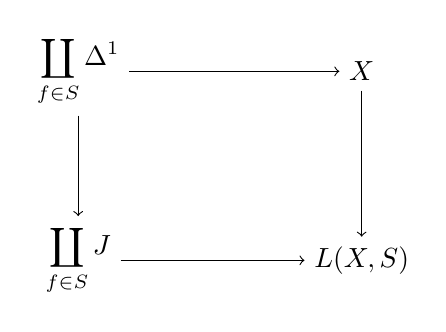
\begin{tikzpicture}
  \node (copd) at (0,0)
    {$\displaystyle\coprod_{f\in S} \Delta^1$};
  \node (x) at (3.6,0) {$X$};
  \node (copj) at (0,-2.4)
    {$\displaystyle\coprod_{f\in S} J$};
  \node (lxs) at (3.6,-2.4) {$L(X, S)$};
  \draw[->] (copd) -- (x);
  \draw[->] (copd) -- (copj);
  \draw[->] (x) -- (lxs);
  \draw[->] (copj) -- (lxs);
\end{tikzpicture}
\end{center}
观察到，如果 $X = \mathcal{C}$ 是一个∞-\trCategory{}，那么 $L(X, S)$ 在%
\trJoyalEquivalence{}意义下等价于 $\mathcal{C}[S^{-1}]$，后者是这样定义的：选取一
个\trInnerAnodyne{}映射 $L(\mathcal{C}, S) \to \mathcal{C}[S^{-1}]$ 以得到一个
∞-\trCategory{}。由于\trInitialVertexMap{}把 $W_X$ 中的一个\trMorphism{}送到 $X$ 中的一条退化
边，显然可以把相应的映射 $\Delta^1 \to X$ 扩充到包含 $\Delta^1 \to J$ 之上。特别
地，我们得到一个诱导映射
$L(\mathrm{N}(\Delta^{\mathrm{op}}_{/X}), W_X) \to X$，并且我们断言，对每个%
\trSimplicialSet{} $X$，这个映射都是一个\trJoyalEquivalence{}。一旦证明了这一点，
定理便由上述观察得证。

我们把从单纯集到\trMarkedSimplicialSet{}的、把 $X$ 送到
$(\mathrm{N}(\Delta^{\mathrm{op}}_{/X}), W_X)$ 的那个\trFunctor{}记为 $F$。我们将
使用下列性质，其验证留作练习：
\begin{enumerate}[label=(\arabic*)]
  \item \trFunctor{} $LF$ 保持\trColimit{}。
  \item \trFunctor{} $LF$ 保持\trMonomorphism{}。
  \item 诸\trInitialVertexMap{}装配成一个\trNaturalTransformation{}%
        $LF \Rightarrow \mathrm{id}$。
\end{enumerate}

现在让我们假设定理对 $\mathcal{C} = \Delta^n$ 已经得证，并设 $X$ 是一个任意的%
\trSimplicialSet{}。我们把 $X$ 写成沿其诸\trSkeleton{} $\mathrm{sk}_n(X)$ 的%
\trColimit{}，从而得到映射
\[
L(\mathrm{N}(\Delta^{\mathrm{op}}_{/X}), W_X)
\cong
\mathrm{colim}_n\,
L(\mathrm{N}(\Delta^{\mathrm{op}}_{/\mathrm{sk}_n(X)}), W_{\mathrm{sk}_n(X)})
\to
\mathrm{colim}_n\, \mathrm{sk}_n(X)
\cong
X,
\]
其中每一步都使用了\trInitialVertexMap{}。所需的图表交换，这一点的证明我们留作练习。如果我们
能证明每个\trInitialVertexMap{}%
\[
L(\mathrm{N}(\Delta^{\mathrm{op}}_{/\mathrm{sk}_n(X)}),
W_{\mathrm{sk}_n(X)})
\to
\mathrm{sk}_n(X)
\]
都是一个\trJoyalEquivalence{}，那么再由另一道练习，同样的结论也适用于上述映射。

接下来，我们对维数 $n$ 作归纳。归纳起点迫使 $X$ 是一些 $\Delta^0$ 的不交并；由于始
顶点映射与不交并可交换，由假设这个映射是一个\trJoyalEquivalence{}。

对于归纳步骤，我们考虑\trPushout{}%
\begin{center}
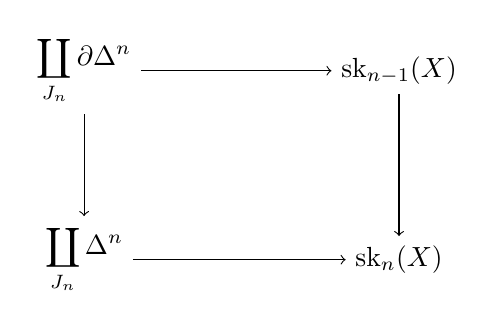
\begin{tikzpicture}
  \node (bd) at (0,0) {$\displaystyle\coprod_{J_n} \partial\Delta^n$};
  \node (skm) at (4,0) {$\mathrm{sk}_{n-1}(X)$};
  \node (dn) at (0,-2.4) {$\displaystyle\coprod_{J_n} \Delta^n$};
  \node (skn) at (4,-2.4) {$\mathrm{sk}_n(X)$};
  \draw[->] (bd) -- (skm);
  \draw[->] (bd) -- (dn);
  \draw[->] (skm) -- (skn);
  \draw[->] (dn) -- (skn);
\end{tikzpicture}
\end{center}
并回忆\trInitialVertexMap{}与\trColimit{}可交换。由归纳与假设，\trInitialVertexMap{}在除右下角之外的各个
角上都是\trJoyalEquivalence{}。然而，由于\trFunctor{}%
$L(\mathrm{N}(\Delta^{\mathrm{op}}_{/(-)}), W_{(-)})$ 保持\trColimit{}与%
\trMonomorphism{}，由\cref{ex:pushout-joyal-equivalence}可知，这个映射也是一个\trJoyalEquivalence{}。

现在我们到达了证明的第二步，在这一步中，我们需要对 $\Delta^n$ 证明定理的陈述。观察
到，在这种情形下，\trInitialVertexMap{}%
\[
\mathrm{N}(\Delta^{\mathrm{op}}_{/\Delta^n}) \to \Delta^n
\]
是\trFunctor{} $\Delta^{\mathrm{op}}_{/\Delta^n} \to [n]$ 在\trNerve{}上诱导的映射，
这个\trFunctor{}把 $f\colon [m] \to [n]$ 送到 $f(0)$。它对\trMorphism{}的作用如下：
给定一个复合 $[k] \to [m] \to [n]$，其中复合是 $g$ 而后一个映射是 $f$，我们需要在
$[n]$ 中找到一个从 $f(0)$ 到 $g(0)$ 的\trMorphism{}。换言之，我们需要证明
$f(0) \le g(0)$。但我们有 $g(0) = f(h(0)) \ge f(0)$，因为 $f$ 与 $h$ 都是单调递增的。

接下来，我们如下构造另一个方向上的\trFunctor{}%
$[n] \to \Delta^{\mathrm{op}}_{/\Delta^n}$：$[n]$ 的\trObject{} $i$ 被送到映射
$\Delta^{\{i,\dotsc,n\}} \to \Delta^n$。显然，如果 $i \le j$，那么存在交换图表
\begin{center}
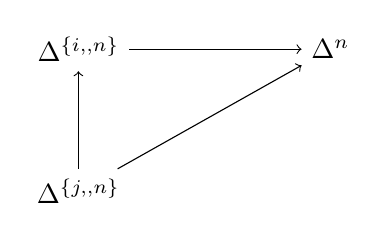
\begin{tikzpicture}
  \node (di) at (0,0) {$\Delta^{\{i,\dotsc,n\}}$};
  \node (dn) at (3.2,0) {$\Delta^n$};
  \node (dj) at (0,-1.8) {$\Delta^{\{j,\dotsc,n\}}$};
  \draw[->] (di) -- (dn);
  \draw[->] (dj) -- (di);
  \draw[->] (dj) -- (dn);
\end{tikzpicture}
\end{center}
从而我们得到一个如所需的\trFunctor{}。可以立即验证，它与\trInitialVertexMap{}的复合由恒等给出。
现在让我们考虑复合
\[
\Delta^{\mathrm{op}}_{/\Delta^n}
\xrightarrow{\ IV\ }
[n]
\xrightarrow{\ i\ }
\Delta^{\mathrm{op}}_{/\Delta^n}.
\]
我们断言，从这个复合 $i \circ IV$ 到恒等\trFunctor{}存在一个典范%
\trNaturalTransformation{}。事实上，这个复合由把 $f\colon [m] \to [n]$ 送到典范包含
$\{f(0), \dotsc, n\} \to [n]$ 给出，其中典范交换三角形
\begin{center}
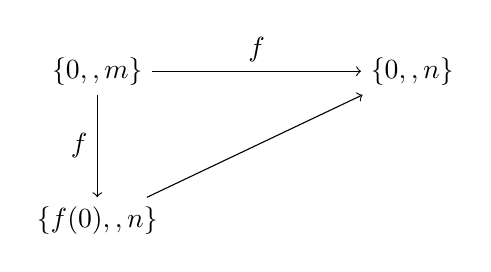
\begin{tikzpicture}
  \node (m0) at (0,0) {$\{0, \dotsc, m\}$};
  \node (n0) at (4,0) {$\{0, \dotsc, n\}$};
  \node (f0) at (0,-1.9) {$\{f(0), \dotsc, n\}$};
  \draw[->] (m0) -- node[above] {$f$} (n0);
  \draw[->] (m0) -- node[left] {$f$} (f0);
  \draw[->] (f0) -- (n0);
\end{tikzpicture}
\end{center}
提供了这个\trNaturalTransformation{}的各分量（左竖直映射）。我们观察到，这些分量全
都含于集合 $W_{\Delta^n}$ 之中。

这一构造提供了单纯集之间的一个映射
\[
\Delta^1 \to
\mathrm{Fun}(\mathrm{N}(\Delta^{\mathrm{op}}_{/\Delta^n}),
\mathrm{N}(\Delta^{\mathrm{op}}_{/\Delta^n}))
\]
它在 $0$ 上限制为 $i \circ IV$、在 $1$ 上限制为恒等。与局部化映射 $\mathrm{N}(\Delta^{\mathrm{op}}_{/\Delta^n}) \to \mathrm{N}(\Delta^{\mathrm{op}}_{/\Delta^n})[W_{\Delta^n}^{-1}]$ 作后合成，并回忆
$i \circ IV$ 把 $W_{\Delta^n}$ 送到诸\trEquivalence{}，我们便得到一个映射
\[
\Delta^1 \to
\mathrm{Fun}(\mathrm{N}(\Delta^{\mathrm{op}}_{/\Delta^n})[W_{\Delta^n}^{-1}],
\mathrm{N}(\Delta^{\mathrm{op}}_{/\Delta^n})[W_{\Delta^n}^{-1}]).
\]
由于上述变换的各分量含于集合 $W_{\Delta^n}$，这个映射是一个\trNaturalEquivalence{}。
于是我们构造了\trFunctor{}%
\[
\mathrm{N}([n]) \to
\mathrm{N}(\Delta^{\mathrm{op}}_{/\Delta^n})[W_{\Delta^n}^{-1}] \to
\mathrm{N}([n]) \to
\mathrm{N}(\Delta^{\mathrm{op}}_{/\Delta^n})[W_{\Delta^n}^{-1}]
\]
使得两个复合都与恒等\trFunctor{}\trNaturalEquivalence{}。因此，\trInitialVertexMap{}正如所愿是
一个\trJoyalEquivalence{}。
\end{proof}

\begin{corollary}\label{cor:straightening}
设 $p\colon \E \to \mathcal{C}$ 是一个\trCocartesianFibration{}。通过逆转上述%
\trEquivalence{}，我们得到一个\trFunctor{}%
\[
\mathcal{C}
\xleftarrow{\ \simeq\ }
\mathrm{N}(\Delta^{\mathrm{op}}_{/\mathcal{C}})[W_\mathcal{C}^{-1}]
\longrightarrow
\mathrm{Cat}_\infty,
\]
称为\trCocartesianFibration{} $p$ 的\trStraightening{}。
\end{corollary}

我们以\trLurie{}的\trStraightening{}--\trUnstraightening{}\trEquivalence{}来结束本节
（不给出它的证明）。非正式地说，它讲的是，\cref{cor:straightening}的\trStraightening{}%
构造诱导出适当的∞-\trCategories{}之间的一个\trEquivalence{}。为了给出一个精确的陈
述，让我们把\trSlice{} $(\mathrm{Cat}_\infty)/\mathcal{C}$ 中由那些为\trCocartesianFibration{}%
$\E \to \mathcal{C}$ 的\trObject{}组成的子范畴记作 $\mathrm{CoCart}(\mathcal{C})$，
其\trMorphism{}是按\cref{def:morphism-of-fibrations}意义下的\trCocartesianFibration{}%
之间的\trMorphism{}。

\begin{theorem}\label{thm:straightening-unstraightening}
对每个∞-\trCategory{} $\mathcal{C}$，存在∞-\trCategories{}之间的一个\trEquivalence{}%
\[
\mathrm{CoCart}(\mathcal{C}) \simeq \mathrm{Fun}(\mathcal{C}, \mathrm{Cat}_\infty).
\]
在\trObject{}上，这个\trEquivalence{}实现的是我们先前的构造。
\end{theorem}

\begin{definition}\label{def:universal-cocartesian-fibration}
考虑∞-\trCategory{} $\mathcal{C} = \mathrm{Cat}_\infty$ 与恒等\trFunctor{}。由%
\cref{thm:straightening-unstraightening}，这对应于 $\mathrm{Cat}_\infty$ 之上的一个%
\trCocartesianFibration{}，称为\emph{\trUniversalCocartesianFibration{}}（universal cocartesian
fibration）。它是一个\trFunctor{} $(\mathrm{Cat}_\infty)_{*\!/} \to \mathrm{Cat}_\infty$，
其中 $(\mathrm{Cat}_\infty)_{*\!/}$ 是一个∞-\trCategory{}，其\trObject{}是诸对
$(\mathcal{C}, x)$，其中 $x$ 是 $\mathcal{C}$ 的一个\trObject{}；而从 $(\mathcal{C}, x)$
到 $(\mathcal{D}, y)$ 的\trMorphism{}由诸对 $(F, \alpha)$ 组成，其中
$F\colon \mathcal{C} \to \mathcal{D}$，而 $\alpha\colon y \to Fx$ 是 $\mathcal{D}$
中的一个\trMorphism{}。
\end{definition}

\begin{remark}\label{rem:under-slice-construction}
构造∞-\trCategory{} $(\mathrm{Cat}_\infty)_{*\!/}$ 并非易事，因为它涉及一个并非严格的
∞-\trCategory{}中的合成。有一些办法可以绕过这个问题，但我们将不在这里深入细节，
见 \cite[Remark 6.1.19]{RV18}。想法是考虑∞-\trCategories{}的单纯\trCategory{}的%
\trCoherentNerve{} $\mathrm{N}(\mathrm{Cat}^1_\infty)$，而不过渡到\trFunctor{}%
\trCategories{}的\trGroupoid{}。这是一个\trSimplicialSet{}，而且人们可以作出它在点
之下的\trSlice{}。结果得到单纯集之间的一个映射
$\mathrm{N}(\mathrm{Cat}^1_\infty)_{\Delta^0/\!/} \to \mathrm{N}(\mathrm{Cat}^1_\infty)$。
由构造，还存在一个\trFunctor{} $\mathrm{Cat}_\infty \to \mathrm{N}(\mathrm{Cat}^1_\infty)$，
而\trSlice{}投射的\trPullback{}结果是一个\trCocartesianFibration{}。
\end{remark}

\begin{remark}\label{rem:pullback-equivalence-rv}
一般地，对每个\trCocartesianFibration{} $\E \to \mathcal{D}$ 与每个∞-\trCategory{}%
$\mathcal{C}$，人们会希望有一个\trFunctor{}%
$\mathrm{Fun}(\mathcal{C}, \mathcal{D}) \to \mathrm{CoCart}(\mathcal{C})$，它在%
\trObject{}上由拉回给定的\trCocartesianFibration{}给出。那么，「$\E \to \mathcal{D}$
是泛的」这一陈述便翻译成「这个\trFunctor{}是∞-\trCategories{}之间的一个%
\trEquivalence{}」这一性质。这样的一个构造在 \cite[Theorem 6.1.13]{RV18} 中完成。
\end{remark}

\begin{remark}\label{rem:straightening-of-functor}
借助\trUniversalCocartesianFibration{}，我们也能说出\trEquivalence{}%
\[
\mathrm{CoCart}(\mathcal{C}) \simeq \mathrm{Fun}(\mathcal{C}, \mathrm{Cat}_\infty)
\]
作用在一个\trFunctor{} $F\colon \mathcal{C} \to \mathrm{Cat}_\infty$ 上给出什么：
它把 $F$ 送到被拉回的\trCocartesianFibration{}%
\[
F^*p\colon F^*(\mathrm{Cat}_\infty)_{*\!/} \to \mathcal{C}.
\]
\end{remark}

下面的引理很快就会对我们有用。

\begin{lemma}\label{lem:fun-preserves-fully-faithful}
设 $f\colon \mathcal{C} \to \mathcal{D}$ 是∞-\trCategories{}之间的一个%
\trFullyFaithful{}\trFunctor{}。那么对任何\trSimplicialSet{} $K$，所诱导的%
\trFunctor{} $\mathrm{Fun}(K, \mathcal{C}) \to \mathrm{Fun}(K, \mathcal{D})$ 仍是%
\trFullyFaithful{}。
\end{lemma}

\begin{proof}
我们首先观察到，一个\trFunctor{} $f$ 是\trFullyFaithful{}，当且仅当图表
\begin{center}
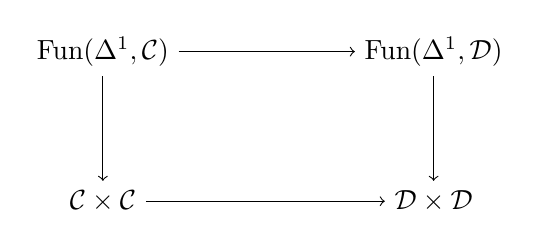
\begin{tikzpicture}
  \node (fc) at (0,0) {$\mathrm{Fun}(\Delta^1, \mathcal{C})$};
  \node (fd) at (4.2,0) {$\mathrm{Fun}(\Delta^1, \mathcal{D})$};
  \node (cc) at (0,-1.9) {$\mathcal{C} \times \mathcal{C}$};
  \node (dd) at (4.2,-1.9) {$\mathcal{D} \times \mathcal{D}$};
  \draw[->] (fc) -- (fd);
  \draw[->] (fc) -- (cc);
  \draw[->] (fd) -- (dd);
  \draw[->] (cc) -- (dd);
\end{tikzpicture}
\end{center}
是\trHomotopyCartesian{}。当把\trFunctor{} $\mathrm{Fun}(K, -)$ 应用到这个图表时，注意它保持%
\trHomotopyCartesian{}图表。利用\trEquivalence{} $\mathrm{Fun}(K, \mathrm{Fun}(\Delta^1, \mathcal{C})) \cong \mathrm{Fun}(\Delta^1, \mathrm{Fun}(K, \mathcal{C}))$，引理得证。
\end{proof}

回忆由第 2 章中的\cref{cor:spc-fully-faithful}，典范\trFunctor{}%
$\mathrm{Spc} \to \mathrm{Cat}_\infty$ 是\trFullyFaithful{}。由%
\cref{lem:fun-preserves-fully-faithful}，对任何∞-\trCategory{} $\mathcal{C}$，
\trFunctor{}%
\[
\mathrm{Fun}(\mathcal{C}, \mathrm{Spc}) \to \mathrm{Fun}(\mathcal{C}, \mathrm{Cat}_\infty)
\]
也是\trFullyFaithful{}。特别地，在上述\trEquivalence{}之下，∞-\trCategory{}%
$\mathrm{Fun}(\mathcal{C}, \mathrm{Spc})$ 必定对应于 $\mathrm{CoCart}(\mathcal{C})$
的某个满子\trCategory{}。这一子\trCategory{}由下述定理给出。

\begin{theorem}\label{thm:lfib-straightening}
对每个∞-\trCategory{} $\mathcal{C}$，\trStraightening{}--\trUnstraightening{}%
\trEquivalence{}限制为一个\trEquivalence{}%
\[
\mathrm{LFib}(\mathcal{C}) \simeq \mathrm{Fun}(\mathcal{C}, \mathrm{Spc}),
\]
其中 $\mathrm{LFib}(\mathcal{C})$ 表示\trSlice{} $(\mathrm{Cat}_\infty)/\mathcal{C}$
中由诸\trLeftFibration{}组成的满子\trCategory{}。
\end{theorem}

\begin{proof}
在\trStraightening{}--\trUnstraightening{}\trEquivalence{}之下，复合
$\mathcal{C} \to \mathrm{Spc} \to \mathrm{Cat}_\infty$ 对应于一个\trCocartesianFibration{}%
$\E \to \mathcal{C}$，其诸\trFibre{}都是∞-\trGroupoid{}。于是，由%
\cref{prop:cartesian-fibration-fibres-groupoids}的对偶版本，$\E \to \mathcal{C}$
是一个\trLeftFibration{}。由于 $\mathcal{C}$ 之上的任何\trMorphism{}%
$\E \to \E'$ 都保持余笛卡尔边（由\cref{lem:cartesian-fibration-right-fibration}，
每条边都是余笛卡尔的），这事实上正如所断言的是该\trSliceCategory{}的\emph{满}子\trCategory{}。
\end{proof}

下述结果几乎就是上述定理的一个推论。

\begin{theorem}\label{thm:spc-slice-straightening}
设 $X$ 是一个∞-\trGroupoid{}。那么\trStraightening{}--\trUnstraightening{}%
\trEquivalence{}限制为一个\trEquivalence{}%
\[
\mathrm{Spc}_{/X} \simeq \mathrm{Fun}(X, \mathrm{Spc}).
\]
\end{theorem}

\begin{proof}
由\cref{thm:lfib-straightening}，我们需要证明存在一个典范\trEquivalence{}%
$\mathrm{LFib}(X) \simeq \mathrm{Spc}_{/X}$。由于 $X$ 是一个∞-\trGroupoid{}，任何%
\trLeftFibration{} $\E \to X$ 事实上都是一个\trKanFibration{}。特别地，$\E$
本身是一个\trKanComplex{}。于是我们发现，\trCategory{} $\mathrm{LFib}(X)$ 是%
\trSlice{} $(\mathrm{Cat}_\infty)/X$ 的满子\trCategory{}，其\trObject{}由诸%
\trKanFibration{}组成。我们得到图表
\begin{center}
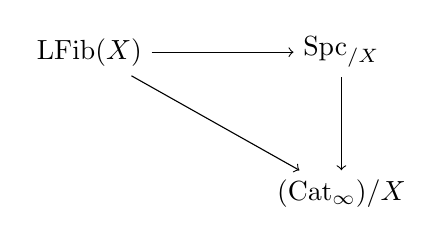
\begin{tikzpicture}
  \node (lf) at (0,0) {$\mathrm{LFib}(X)$};
  \node (spc) at (3.2,0) {$\mathrm{Spc}_{/X}$};
  \node (slice) at (3.2,-1.8) {$(\mathrm{Cat}_\infty)/X$};
  \draw[->] (lf) -- (spc);
  \draw[->] (lf) -- (slice);
  \draw[->] (spc) -- (slice);
\end{tikzpicture}
\end{center}
\trFunctor{} $\mathrm{Spc}_{/X} \to (\mathrm{Cat}_\infty)/X$ 是\trFullyFaithful{}，
因为由第 2 章中的\cref{cor:spc-fully-faithful}，\trFunctor{}%
$\mathrm{Spc} \to \mathrm{Cat}_\infty$ 是\trFullyFaithful{}，另见%
\cref{cor:slice-fully-faithful}。由此得出，\trFunctor{}%
$\mathrm{LFib}(X) \to \mathrm{Spc}_{/X}$ 也是\trFullyFaithful{}。此外，
∞-\trGroupoid{}之间的任何映射 $Y \to X$ 都等价于一个\trKanFibration{}。这蕴含包含
$\mathrm{LFib}(X) \to \mathrm{Spc}_{/X}$ 是\trEssentiallySurjective{}且%
\trFullyFaithful{}，从而正如所需是一个\trEquivalence{}。
\end{proof}

在我们能够建立\cref{cor:slice-fully-faithful}——完成上述证明所需要——之前，我们将
需要下面对切片∞-\trCategories{}中诸\trMappingSpace{}的分析。这一陈述稍后还会再次用
到。其对偶版本是 \cite[Lemma 5.5.5.12]{Lur09}。

\begin{proposition}\label{prop:mapping-space-slice}
设 $\mathcal{C}$ 是一个∞-\trCategory{}，并设 $f\colon x \to z$ 与
$g\colon y \to z$ 是 $\mathcal{C}$ 中的\trMorphism{}，视为 $\mathcal{C}_{/z}$ 的%
\trObject{}。那么图表
\begin{center}
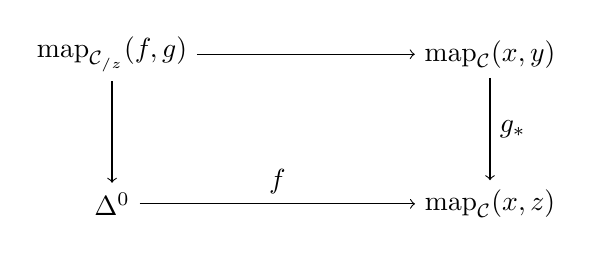
\begin{tikzpicture}
  \node (mfg) at (0,0) {$\mathrm{map}_{\mathcal{C}_{/z}}(f, g)$};
  \node (mxy) at (4.8,0) {$\mathrm{map}_{\mathcal{C}}(x, y)$};
  \node (d0) at (0,-1.9) {$\Delta^0$};
  \node (mxz) at (4.8,-1.9) {$\mathrm{map}_{\mathcal{C}}(x, z)$};
  \draw[->] (mfg) -- (mxy);
  \draw[->] (mfg) -- (d0);
  \draw[->] (mxy) -- node[right] {$g_*$} (mxz);
  \draw[->] (d0) -- node[above] {$f$} (mxz);
\end{tikzpicture}
\end{center}
是\trHomotopyCartesian{}。
\end{proposition}

\begin{proof}
回忆映射 $g_*\colon \mathrm{map}_\mathcal{C}(x, y) \to \mathrm{map}_\mathcal{C}(x, z)$%
\footnote{译注：原书印作「$\mathrm{map}_{\mathcal{C}}(x,y) \to \mathrm{map}_{\mathcal{C}}(y,z)$」，据命题陈述与证明末项，此处应为 $\mathrm{map}_{\mathcal{C}}(x,z)$，兹径改。——译者注}
是如下构造的。我们有两个典范的限制\trFunctor{}%
\[
\mathcal{C}_{/y}
\xleftarrow{\ \simeq\ }
\mathcal{C}_{/g}
\to
\mathcal{C}_{/z},
\]
其中第一个是一个\trEquivalence{}。逆转这个\trEquivalence{}并在 $\mathcal{C}$ 中取
$x$ 之上的诸\trFibre{}，我们得到
\[
\mathcal{C}_{/y} \times_\mathcal{C} \{x\}
\simeq
\mathcal{C}_{/g} \times_\mathcal{C} \{x\}
\to
\mathcal{C}_{/z} \times_\mathcal{C} \{x\},
\]
其中首项与末项分别由 $\mathrm{map}^R_\mathcal{C}(x, y)$ 与
$\mathrm{map}^R_\mathcal{C}(x, z)$ 给出。接着我们考虑图表
\begin{center}
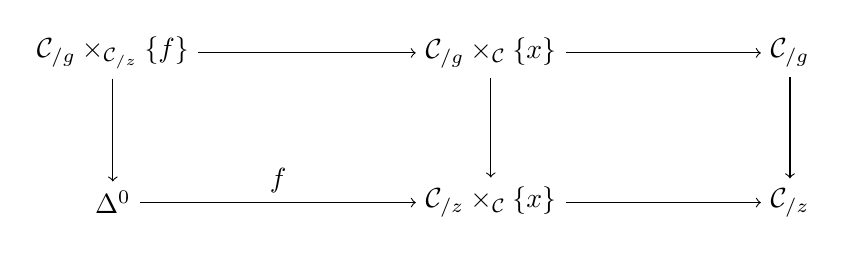
\begin{tikzpicture}
  \node (tl) at (0,0) {$\mathcal{C}_{/g} \times_{\mathcal{C}_{/z}} \{f\}$};
  \node (tm) at (4.8,0) {$\mathcal{C}_{/g} \times_\mathcal{C} \{x\}$};
  \node (tr) at (8.6,0) {$\mathcal{C}_{/g}$};
  \node (bl) at (0,-1.9) {$\Delta^0$};
  \node (bm) at (4.8,-1.9) {$\mathcal{C}_{/z} \times_\mathcal{C} \{x\}$};
  \node (br) at (8.6,-1.9) {$\mathcal{C}_{/z}$};
  \draw[->] (tl) -- (tm);
  \draw[->] (tm) -- (tr);
  \draw[->] (tl) -- (bl);
  \draw[->] (tm) -- (bm);
  \draw[->] (tr) -- (br);
  \draw[->] (bl) -- node[above] {$f$} (bm);
  \draw[->] (bm) -- (br);
\end{tikzpicture}
\end{center}
其中右边的正方形与大正方形都是\trPullback{}。因此，所有正方形都是\trPullback{}。
此外，由于最右边的竖直映射是一个\trRightFibration{}，中间的竖直映射是一个其目标为
∞-\trGroupoid{}的\trRightFibration{}。于是，中间的竖直映射是一个\trKanFibration{}，
并且为与 $g$ 作后合成所得的映射提供了一个模型。尚需证明存在一个典范\trEquivalence{}%
\footnote{译注：原书下式右端印作
$\mathcal{C}_{/g} \times_{\mathcal{C}_{/z}} \times \{f\}$，多出一个 $\times$；
按上图左上角，此拉回应为
$\mathcal{C}_{/g} \times_{\mathcal{C}_{/z}} \{f\}$，兹径改。——译者注}
\[
\mathrm{map}_{\mathcal{C}_{/z}}(f, g) \simeq
\mathcal{C}_{/g} \times_{\mathcal{C}_{/z}} \{f\}.
\]
为此，我们观察到 $(\mathcal{C}_{/z})_{/g} \cong \mathcal{C}_{/g}$，故断言得证。
\end{proof}

\begin{corollary}\label{cor:slice-fully-faithful}
设 $\mathcal{C} \subseteq \mathcal{D}$ 是一个满子\trCategory{}，并设 $z$ 是
$\mathcal{C}$ 的一个\trObject{}。那么典范\trFunctor{}%
$\mathcal{C}_{/z} \to \mathcal{D}_{/z}$ 仍是\trFullyFaithful{}。
\end{corollary}

\begin{proof}
设 $f\colon x \to z$ 与 $g\colon y \to z$ 是 $\mathcal{C}_{/z}$ 的\trObject{}。我们
希望证明映射
\[
\mathrm{map}_{\mathcal{C}_{/z}}(f, g) \to
\mathrm{map}_{\mathcal{D}_{/z}}(f, g)
\]
是一个\trHomotopyEquivalence{}。由\cref{prop:mapping-space-slice}，只需证明在图表
\begin{center}
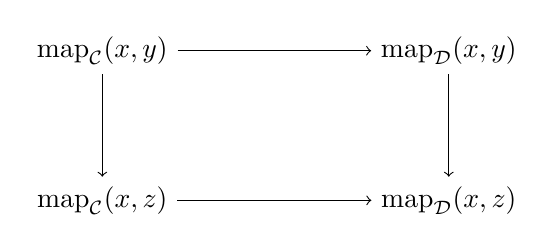
\begin{tikzpicture}
  \node (tl) at (0,0) {$\mathrm{map}_\mathcal{C}(x, y)$};
  \node (tr) at (4.4,0) {$\mathrm{map}_\mathcal{D}(x, y)$};
  \node (bl) at (0,-1.9) {$\mathrm{map}_\mathcal{C}(x, z)$};
  \node (br) at (4.4,-1.9) {$\mathrm{map}_\mathcal{D}(x, z)$};
  \draw[->] (tl) -- (tr);
  \draw[->] (tl) -- (bl);
  \draw[->] (tr) -- (br);
  \draw[->] (bl) -- (br);
\end{tikzpicture}
\end{center}
中两个水平映射都是\trEquivalence{}。但这由「包含
$\mathcal{C} \subseteq \mathcal{D}$ 是\trFullyFaithful{}」这一假设得出。%
\footnote{译注：原书此处印作「由假设 $f$ 是全忠实的得出」，但本证明中的 $f$ 是
$\mathcal{C}_{/z}$ 的对象（$\mathcal{C}$ 中的\trMorphism{} $x \to z$），并非该假设
的合适主体；按陈述，此假设应为包含 $\mathcal{C} \to \mathcal{D}$ 全忠实（即
$\mathcal{C} \subseteq \mathcal{D}$ 为满子\trCategory{}），兹径改。——译者注}
\end{proof}
